\section*{Introduction}

\begin{frame}{Introduction}
\begin{itemize}
\item Dans les images de zoo, difficile d'éviter les grillages : \emph{post-traitement} des images pour essayer de retirer grillage, nécessité de reconstruire l'objet caché.
\item Grillage a des propriétés remarquables : composé de lignes, angles quasi-horizontaux, couleur presque uniforme...
\end{itemize}
\begin{block}{Approche retenue}
Traitement automatique des images de zoo basé - essentiellement - sur la structure spatiale du grillage qui créé une image \og démasquée\fg.
\end{block}
\end{frame}




\section{Hypothèses}

\begin{frame}{Hypothèses}
\begin{description}
\item[Grillage non flou. ]Détection de contour nécessite que le grillage soit un minimum net.

\item[Grillage sans trop de perspective. ]Si il y une trop forte homothétie appliquée au grillage, l'espacement dans la transformation de Hough n'est plus régulier.

\item[Grillage sans rupture de direction ou double grillage. ]L'algorithme ne détecte qu'une forme de grillage.

\item[Grillage total. ]Masque étendu sur toute l'image.

\item[Grillage sans \og croisillons\fg. ]Les lignes sont décalées à chaque intersection.

\item[Nombre minimal de barreaux. ]La photo possède au moins deux barreaux dans chaque direction.
\end{description}
\end{frame}



\section{Détection de contours et extraction de lignes}

\subsection{Détection de contours}

\begin{frame}{Détecteur de contours}
\begin{block}{Première étape de l'algorithme}
Détecter les contours dans l'image. Idée : les grillages interviennent comme des bords.
\end{block}
Filtre de Canny utilisé, échelle de précision pendant le filtrage Gaussien. Possibilités :
\begin{enumerate}
\item Adapter variance de la gaussienne à la taille caractéristique du grillage ;
\item redimensionner les images pour que les grillages ait une taille - à peu près - fixe entre plusieurs images. 
\end{enumerate}
Lenteur de l'\emph{inpainting} sur grandes images $\Rightarrow$ choix 2.
\end{frame}

\begin{frame}{Détecteur de contours}
\begin{figure}[ht!]
\centering
\begin{tabular}{cc}
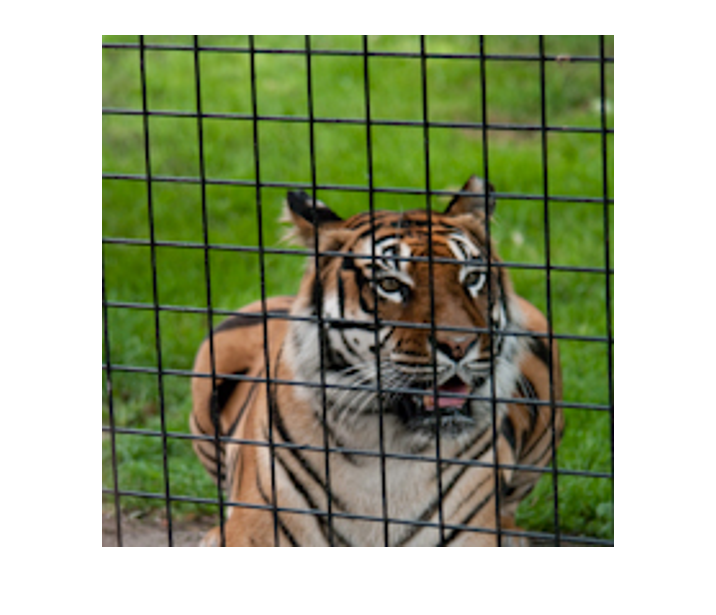
\includegraphics[width = .5\columnwidth]{fig/tigre_rescale.png} &
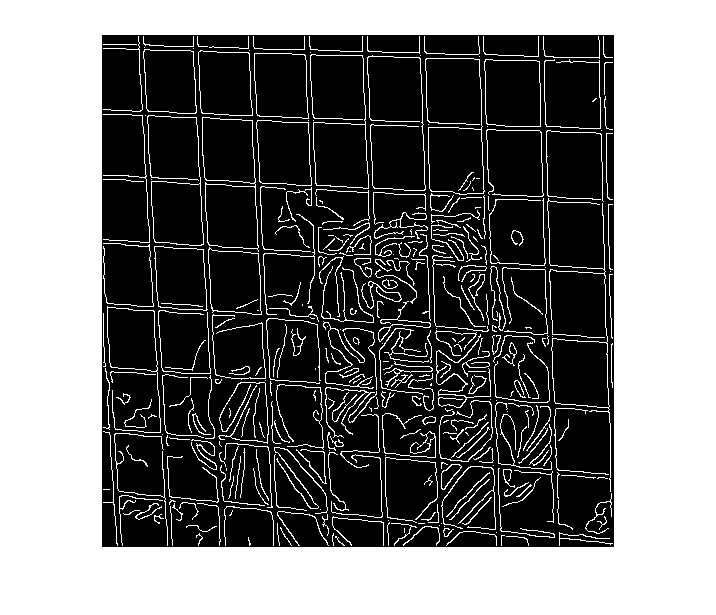
\includegraphics[width = .5\columnwidth]{fig/contour.png} 
\end{tabular}
\caption{Dans les colonnes de gauche, l'image initiale et dans celles de droite les résultats de la détection de contour avec l'algorithme de Canny. Toutes les images sont redimensionnées en $512\times 512$. }
\end{figure}
\end{frame}


\begin{frame}{Détecteur de contours}
\begin{figure}[ht!]
\centering
\begin{tabular}{cc}
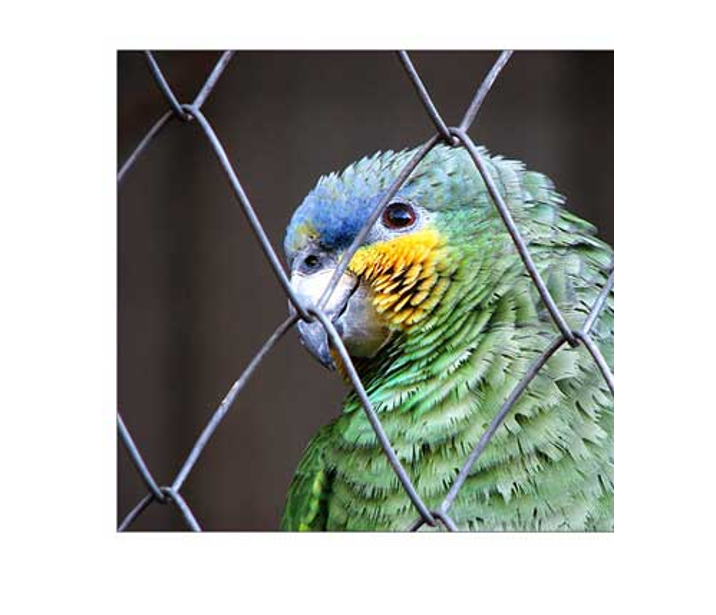
\includegraphics[width = .5\columnwidth]{fig/parrot_rescale.png} &
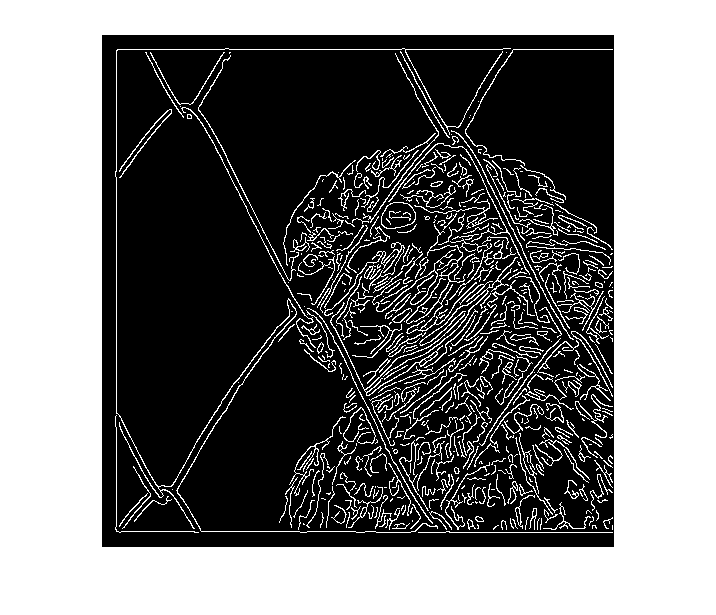
\includegraphics[width = .5\columnwidth]{fig/contour_parrot.png}
\end{tabular}
\caption{Dans les colonnes de gauche, l'image initiale et dans celles de droite les résultats de la détection de contour avec l'algorithme de Canny. Toutes les images sont redimensionnées en $512\times 512$. }
\end{figure}
\end{frame}


\begin{frame}{Détecteur de contours}
\begin{figure}[ht!]
\centering
\begin{tabular}{cc}
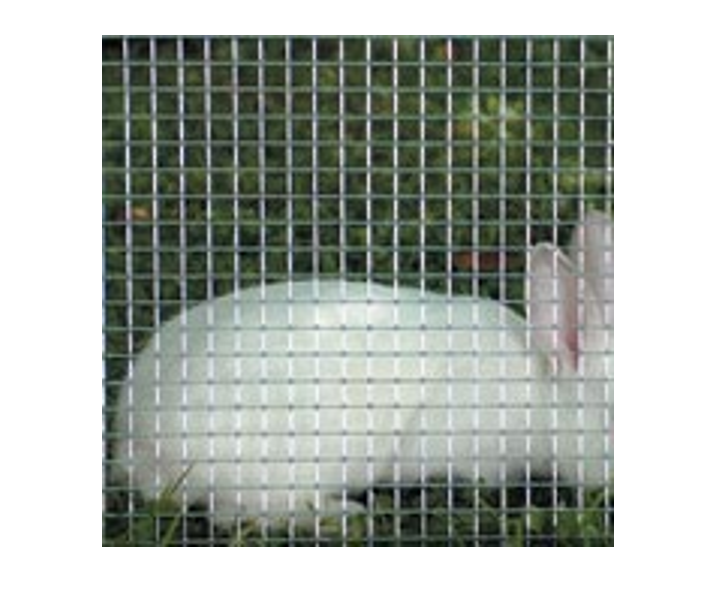
\includegraphics[width = .5\columnwidth]{fig/lapin_rescale.png} &
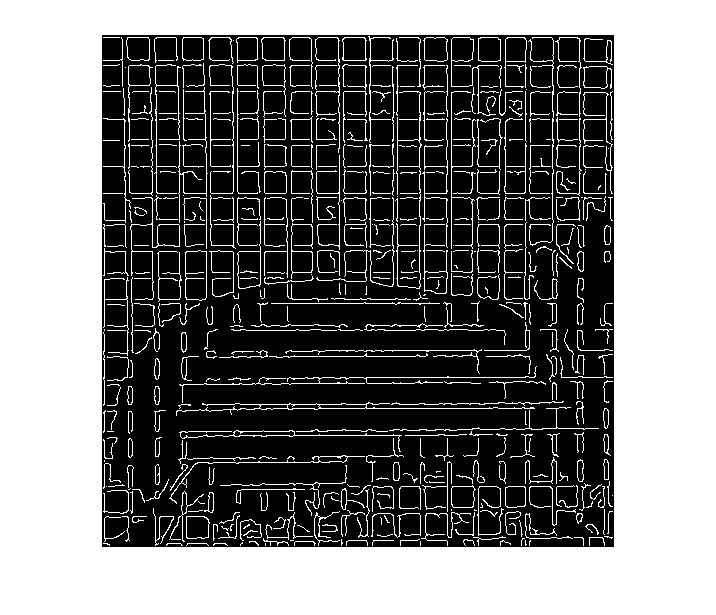
\includegraphics[width = .5\columnwidth]{fig/contour_lapin.png}
\end{tabular}
\caption{Dans les colonnes de gauche, l'image initiale et dans celles de droite les résultats de la détection de contour avec l'algorithme de Canny. Toutes les images sont redimensionnées en $512\times 512$. }
\end{figure}
\end{frame}


\subsection{Extraction de lignes}

\begin{frame}{Extraction de lignes}
\begin{block}{Deuxième étape de l'algorithme}
Extraire les lignes à partir de la détection de contour
\end{block}
On utilise pour ceci la transformation de Hough.
\begin{itemize}
\item utilise une représentation des droite : 
\begin{equation}
r = x \cos \theta + y \sin\theta
\end{equation}
\item A chaque point est associé une courbe - sinusoïde - dans l'espace de Hough. 
\item Croisement de deux courbes $\Rightarrow$ droite reliant les deux points liés à ces courbes.
\end{itemize} 
\end{frame}


\begin{frame}{Extraction de lignes}
\begin{figure}[ht!]
\centering
\begin{tabular}{cc}
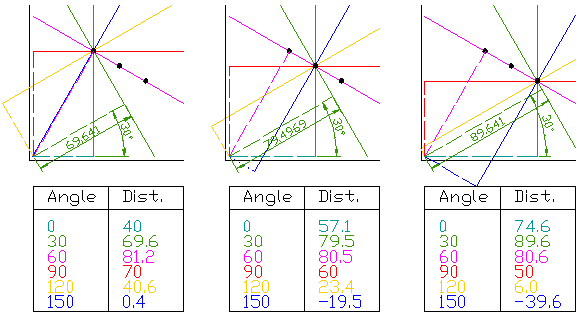
\includegraphics[width = .5\columnwidth]{fig/Hough_transform_diagram.png} &
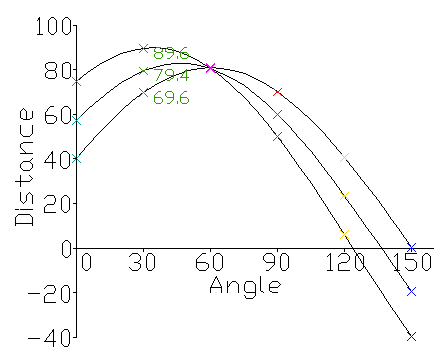
\includegraphics[width = .5\columnwidth]{fig/Hough_space_plot_example.png}
\end{tabular}
\caption{Transformation de Hough, les croisements dans l'espace arrivé correspondent aux droites dans l'image initiale. }
\end{figure}
\end{frame}
